
\documentclass[paper=a4, fontsize=11pt]{scrartcl} % A4 paper and 11pt font size

\usepackage[T1]{fontenc} % Use 8-bit encoding that has 256 glyphs
\usepackage{fourier} % Use the Adobe Utopia font for the document - comment this line to return to the LaTeX default
\usepackage[english]{babel} % English language/hyphenation
\usepackage{amsmath,amsfonts,amsthm} % Math packages
\usepackage{tabularx}
\usepackage{outlines}
\usepackage{framed,varwidth}
\usepackage{enumitem}
\usepackage{lipsum} % Used for inserting dummy 'Lorem ipsum' text into the template
\usepackage[left=0.5in, right=0.5in, top=3in, bottom=.25in]{geometry}
\geometry{}
\usepackage{sectsty} % Allows customizing section commands
\usepackage{graphicx}
\usepackage{fancyhdr} % Custom headers and footers


\sectionfont{\centering \normalfont\scshape} % Make all sections centered, the default font and small caps
\pagestyle{fancyplain} % Makes all pages in the document conform to the custom headers and footers
\fancyhead{} % No page header - if you want one, create it in the same way as the footers below
\fancyfoot[L]{} % Empty left footer
\fancyfoot[C]{} % Empty center footer
\fancyfoot[R]{\thepage} % Page numbering for right footer
\renewcommand{\headrulewidth}{0pt} % Remove header underlines
\renewcommand{\footrulewidth}{0pt} % Remove footer underlines
\setlength{\headheight}{0pt} % Customize the height of the header

\numberwithin{equation}{section} % Number equations within sections (i.e. 1.1, 1.2, 2.1, 2.2 instead of 1, 2, 3, 4)
\numberwithin{figure}{section} % Number figures within sections (i.e. 1.1, 1.2, 2.1, 2.2 instead of 1, 2, 3, 4)
\numberwithin{table}{section} % Number tables within sections (i.e. 1.1, 1.2, 2.1, 2.2 instead of 1, 2, 3, 4)

\graphicspath{{./}}
%\setlength\parindent{0pt} % Removes all indentation from paragraphs - comment this line for an assignment with lots of text

\makeatletter
	\newcommand*\variableheghtrulefill[1][.4\p@]
	{%
		\leavevmode
		\leaders \hrule \@height #1\relax \hfill
		\null
	}
\makeatother

%----------------------------------------------------------------------------------------
%	TITLE SECTION
%----------------------------------------------------------------------------------------

\newcommand{\horrule}[1]{\rule{\linewidth}{#1}} % Create horizontal rule command with 1 argument of height
% \title{Template: Homework 1}
\title{	
\normalfont \normalsize 
%\textsc{Rutgers University, Real Analysis I} \\ [25pt] % Your university, school and/or department name(s)
\horrule{0.5pt} \\[0.4cm] % Thin top horizontal rule
\huge CMPSC 360: Homework 02 \\ % The assignment title
\horrule{2pt} \\[0.5cm] % Thick bottom horizontal rule
}

\author{\textbf{\underline{Name:}}Kyle Salitrik | \textit{\textbf{\underline{ID\#:}} 997543474} | \textit{\textbf{\underline{PSU ID:}} kps168}} % Your name

\date{\normalsize\today} % Today's date or a custom date

\begin{document}

\maketitle % Print the title

%----------------------------------------------------------------------------------------
%	PROBLEM 1
%----------------------------------------------------------------------------------------
\newgeometry{top=.75in, bottom=.75in, left=1.25in,right=1.25in}
\section*{\variableheghtrulefill[.25ex]\quad Problem 1 \quad\variableheghtrulefill[.25ex]}

\begin{center}
  \fbox{\quad%
    \begin{varwidth}{\linewidth}
    	Explain how propositional states can be applicable for translating discrete math into the automata systems for the robot applicable to workshop safety using a hash function? 
    \end{varwidth}%
  \quad}
\end{center}

\quad Propositional states can be used by implementing sensor conditions and known data in order to automate a robot to perform tasks. For this example, the robot must know if the sensor detects an object on the ground, then it must go and pick the object up which can be implemented by discreet functions.

%----------------------------------------------------------------------------------------
%	PROBLEM 2
%----------------------------------------------------------------------------------------
\section*{\variableheghtrulefill[.25ex]\quad Problem 2 \quad\variableheghtrulefill[.25ex]}

\begin{center}
  \fbox{\quad%
    \begin{varwidth}{\linewidth}
    	Write each propositional state that represents the described situation.
    \end{varwidth}%
  \quad}
\end{center}

\begin{outline}
\1 States:
	\2 A: Robot locates object
	\2 B: Robot picks up object
	\2 C: Robot loses 4 points
	\2 D: Robot gains 10 points
	\2 E: Person steps on object
	\2 F: Person has stopped walking
	\2 G: Person restarts walking
	\2 H: Person is slower than robot
	\2 I: Robot increases speed
	\2 J: Robot does not increase speed
\1 Propositions:
	\2 Robot locates an object and must pick it up. $A \implies B$
	\2 Robot locates an object, picks it up and gains points. $(A \land B) \implies D$
	\2 Person steps on an object the robot has not picked up and the robot loses points. $(\neg B \land E) \implies C$
	\2 Person stops walking and restarts, but is slower than the robot. $(F \land G \land H) \implies J$
	\2 Person stops walking and restarts, but is faster than the robot. $(F \land G \land \neg H) \implies I$
\end{outline}

\newpage
%----------------------------------------------------------------------------------------
%	PROBLEM 3
%----------------------------------------------------------------------------------------
\section*{\variableheghtrulefill[.25ex]\quad Problem 3 \quad\variableheghtrulefill[.25ex]}

\begin{center}
  \fbox{\quad%
    \begin{varwidth}{\linewidth}
    	Write each propositional state that represents the described situation.
    \end{varwidth}%
  \quad}
\end{center}

\makebox[\textwidth][l]{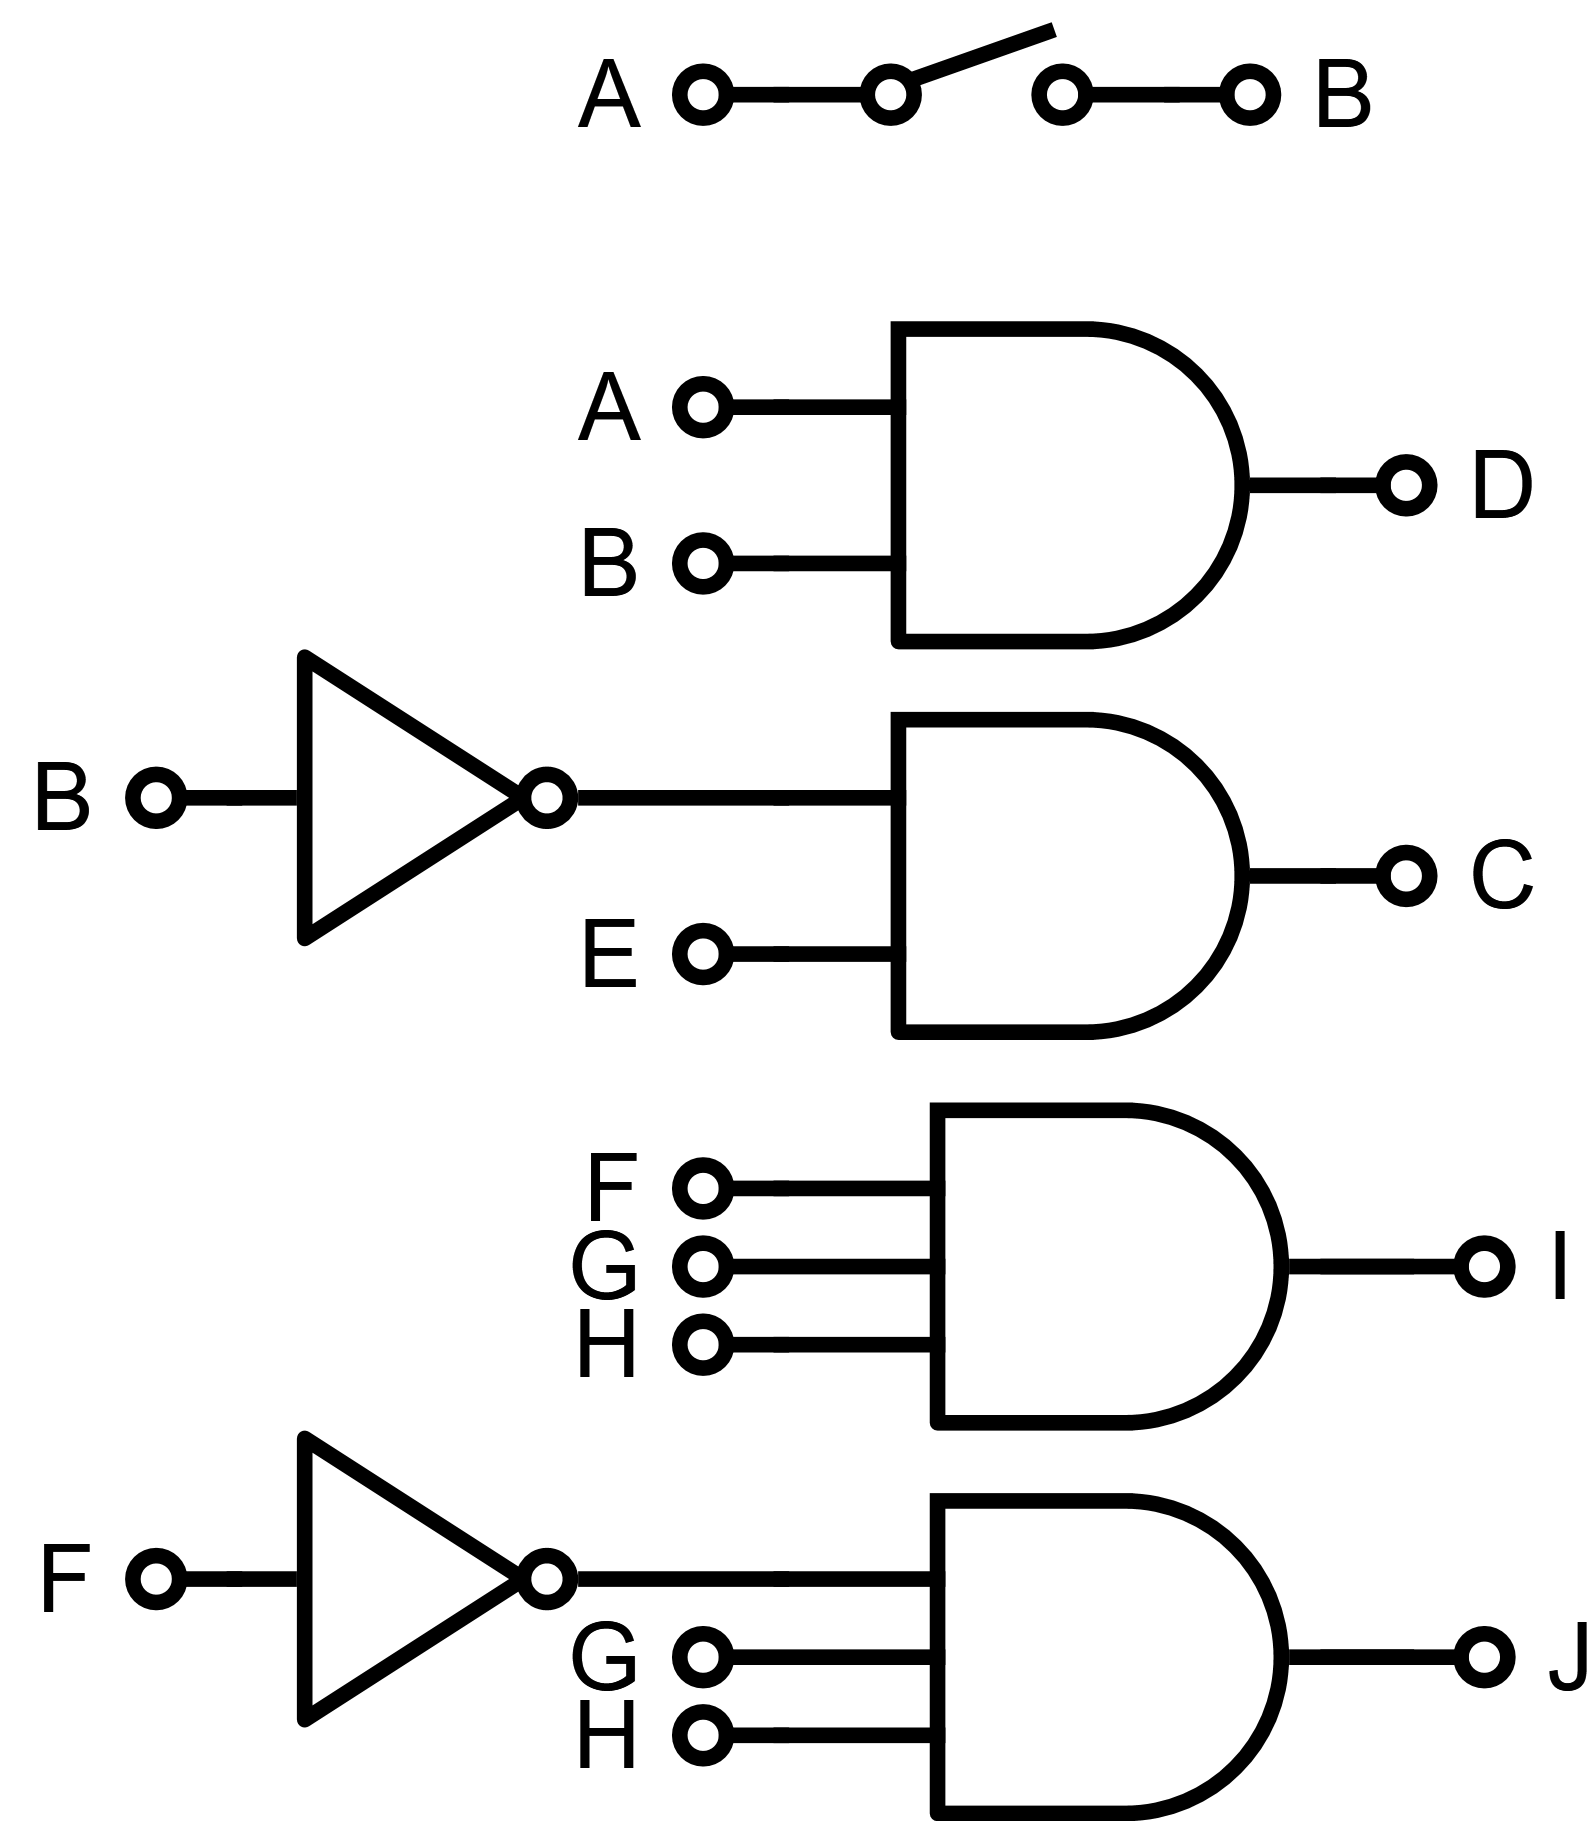
\includegraphics[width=.5\pagewidth]{circuits.png}}

\end{document}